\section{Evaluation}

%TODO: Be consistent about machine vs. target.
%TODO: Say that atoms and targets are interchangeable.
%TODO: Maybe add a few examples from Chimera/Bohatei on security.
%TODO: Mihai: Add figure of CONGA's SCC here maybe?
%TODO: Try and get an atom for CoDel and trTCM.

\label{s:eval}

\begin{table}[!t]
  \begin{scriptsize}
  \begin{tabular}{|p{0.08\textwidth}|p{0.31\textwidth}|p{0.03\textwidth}|}
    \hline
    Atom & Description & Area (sq. microns)\\
    Stateless & Arithmetic, logic, relational, and conditional operations on packet/constant operands & 1383 \\
    \hline
    Read/Write & Read/Write packet field/constant into single state variable. & 249 \\
    \hline
    ReadAddWrite (RAW) & Add packet field/constant to state variable (OR) Write packet field/constant into state variable. & 430 \\
    \hline
    Predicated ReadAddWrite (RAW) & Execute RAW on state variable only if a predicate is true, else leave unchanged. & 790 \\
    \hline
    IfElse ReadAddWrite (IfElseRAW) & Execute two separate RAWs: one each for when a predicate is true or false. & 985 \\
    \hline
    Subtract (Sub) & Same as IfElseRAW, but also allow subtracting a packet field/constant. & 1301 \\
    \hline
    Nested Ifs (Nested) & Same as Sub, but with an additional level of nesting that provides 4-way predication. & 3091 \\
    \hline
    Paired updates (Pairs) & Same as Nested, but allow updates to a pair of state variables, where predicates can use both state variables. & 4440 \\
    \hline
  \end{tabular}
  \end{scriptsize}
  \caption{Atoms with their area overhead in a 32 nm standard-cell library.
  All atoms meet timing at 1GHz. Each of the seven compiler targets contains
  one of the seven stateful atoms above and the single stateless atom.}
  \label{tab:templates}
\end{table}

\begin{table*}[!t]
  \begin{tabular}{|p{0.14\textwidth}|p{0.43\textwidth}|p{0.08\textwidth}|p{0.06\textwidth}|p{0.07\textwidth}|p{0.06\textwidth}|p{0.03\textwidth}|}
\hline
Algorithm & Description & Least expressive atom & Pipeline depth, width & Ingress or Egress Pipeline? & Domino LOC & P4 LOC \\
\hline
\pbox{0.16\textwidth}{Bloom filter~\cite{bloom}\\(3 hash functions)} & \pbox{0.54\textwidth}{Set membership bit on every packet.} & Write & 4, 3 & Either & 29 & 104 \\
\hline
\pbox{0.16\textwidth}{Heavy Hitters~\cite{opensketch}\\(3 hash functions)} & Increment Count-Min Sketch~\cite{cormode} on every packet. & RAW & 10, 9 & Either & 35 & 192  \\
\hline
Flowlets~\cite{flowlets} & Update saved next hop if flowlet threshold is exceeded. & PRAW & 6, 2 & Ingress & 37 & 292 \\
\hline
RCP~\cite{rcp} & \pbox{0.44\textwidth}{Accumulate RTT sum if\\RTT is under maximum allowable RTT.} & PRAW & 3, 3 & Egress & 23 & 75\\
\hline
\pbox{0.16\textwidth}{Sampled\\NetFlow~\cite{sampled_nflow}} & \pbox{0.47\textwidth}{Sample a packet if packet count reaches N;\\Reset count to 0 when it reaches N.} & IfElseRAW & 4, 2 & Either  & 18 & 70\\
\hline
HULL~\cite{hull} & Update counter for virtual queue. & Sub & 7, 1 & Egress & 26 & 95 \\
\hline
\pbox{0.16\textwidth}{Adaptive\\Virtual Queue~\cite{avq}} & Update virtual queue size and virtual capacity & Nested & 7, 3 & Ingress & 36 & 147 \\
\hline
CONGA~\cite{conga} & \pbox{0.54\textwidth}{Update best path's utilization/id if we see a better path.\\
                                           Update best path utilization alone if it changes.}  & Pairs & 4, 2 & Ingress & 32 & 89 \\
\hline
%trTCM~\cite{trTCM} & Update token counts for each token bucket & Doesn't map & 7, 3 & Either \\
%\hline
%CoDel~\cite{codel} & \pbox{0.54\textwidth}{Update:\\Whether we are marking or not.\\Time for next mark.\\Number of marks so far.\\Time at which min. queuing delay will exceed target.}& Doesn't map & 15, 3 & Egress \\
%\hline
\end{tabular}
\caption{Data-plane algorithms}
\label{tab:algos}
\end{table*}

First, we evaluate \pktlanguage's expressiveness by using it to write
data-plane algorithms and comparing it to how they would be written in P4
(Table~\ref{tab:algos}). We then design a set of \absmachine machines
(Table~\ref{tab:templates}) that serve as compiler targets for \pktlanguage.
These machines are readily feasible in today's transistor technology and their
atoms incur modest chip area overhead relative to a baseline switch chip. Next,
we use the \pktlanguage compiler to compile the programs in
Table~\ref{tab:algos} to the targets in Table~\ref{tab:templates}.  We conclude
by showing a tradeoff between a target's programmability (the space of
data-plane algorithms that it can run at line rate) and the target's
performance (the maximum line rate it can support).

\subsection{Expressiveness}
\label{ss:Expressiveness}

To evaluate \pktlanguage's expressiveness, we express several data-plane
algorithms (Table~\ref{tab:algos}) in \pktlanguage. These algorithms encompass
a variety of data-plane functionality including data-plane load balancing,
in-network congestion control, active queue management, and measurement. In
addition, \pktlanguage has been used for programmable
scheduling~\cite{prog_sched_arxiv}.  In all these cases, the algorithms are
naturally expressed as blocks of imperative code and translating them to
\pktlanguage syntax was straightforward.

By contrast, expressing one of these algorithms in P4 requires manually teasing
out portions of the algorithm that can reside in independent match-action
tables and then chaining these tables together. In essence, the programmer
carries out the transformations in \pktlanguage's compiler, which is both
tedious (as measured by line of code (LOC) counts) and error prone (in terms of
maintaining correctness).

\paragraph{Quantitative comparison against P4} Of the algorithms in
Table~\ref{tab:algos}, only flowlet switching has a hand-written P4
implementation~\cite{p4_flowlet}. This implementation requires 292 lines of
uncommented P4, in comparison to the 37 lines of \pktlanguage in
Figure~\ref{fig:flowlet_code}. It also requires the programmer to manually
specify tables, how they are chained, what headers are required, and how they
are parsed.

Further, the same implementation is only guaranteed to be correct on a software
switch because it requires synchronized access to the saved\_hop variable from
two adjacent pipeline stages, which requires locking that is challenging at
line rate. This illustrates the additional programmer burden when programming
with P4. Reasoning about how state variables should be distributed across a
pipeline is error prone and is best moved into a compiler where all algorithms
can benefit from it.

% Keep this?
Ideally, we could repeat the same comparison with P4 for all other algorithms.
But, perhaps in part due to the difficulty of manually writing stateful
algorithms in P4, these algorithms don't have P4 counterparts today. To address
this, we wrote a backend for \pktlanguage that generated P4 from \pktlanguage
by turning every codelet into a default action~\cite{p4spec}.  We report the
number of lines of code in the autogenerated P4 programs in
Table~\ref{tab:algos} and compare them with programs written in
\pktlanguage. While the LOC count could be lesser for manually written P4
programs, our overall message is simple: for stateful data-plane algorithms,
coding in \pktlanguage is easier relative to P4 and results in more concise
(between 3 and 8$\times$) and correct code.

%Anirudh: Chang felt this was incidental.
%%We did, however, modify CoDel. CoDel is a head-drop active queue
%%management scheme, which uses a loop~\cite{codel_code} to repeatedly dequeue
%%packets until it can send one out.  We replaced the while loop with an if
%%statement and mark dequeued packets instead of dropping them. A line-rate
%%switch can dequeue only once per packet. Dropping these dequeued packets,
%%instead of marking them, leads to an idle line and wasted capacity.

\subsection{Compiler targets}
\label{ss:targets}

We design a concrete set of compiler targets for \pktlanguage based on the
\absmachine machine model. First, we specify computational limits on atoms in
each compiler target using atom templates. By expressing these atoms as digital
circuits, we quantify the area of each atom in a 32 nm standard-cell library
when running at 1GHz using the Synopsys Design Compiler~\cite{synopsys_dc}.
Second, using an individual atom's area and a switching chip's
area~\cite{gibb_parsing}, we determine resource limits on the number of atoms
in each stage and the number of stages in a pipeline.

\paragraph{Computational limits}
An atom's computational limits dictate what algorithms can or can't be run on
the \absmachine machine at line rate. Stateless atoms are easier to design
because any stateless operation can be spread out across multiple stages of the
pipeline without violating atomicity~(\S\ref{ss:atoms}). We design a stateless
atom that can support simple arithmetic (add, subtract, left shift, right
shift), logical (and, or, xor), relational (>=, <=, ==, !=), or conditional
operations ( C's ``?'' operator) on a set of packet fields. Any packet field
can also be substituted with a constant operand. The resulting circuit meets
timing at 1GHz and occupies an area of 1383 square microns.

Designing stateful atoms is more involved because it is tied to which
algorithms the switch wants to support at line rate. A more complex stateful
atom can support more data-plane algorithms (we quantify this in the next
section), but, at the same time, incurs greater area overhead. To illustrate
this, we design a containment hierarchy of stateful atoms, where each atom can
express all stateful operations that could be expressed by its predecessor
(Table~\ref{tab:templates}). Again, the resulting circuits meet timing at 1 GHz
and occupy varying amounts of area depending on their complexity.

\paragraph{Resource limits}
Now that we have a single stateless atom and multiple stateful atoms, we can
design compiler targets using these atoms.  We design one compiler target for
each combination of a stateful atom in Table~\ref{tab:templates} along with the
single stateless atom. We determine resource limits for stateful and stateless
atoms separately.

For the stateless atom, assuming a switch chip's area is 200 $mm^2$ (this is
the smallest chip area given by Gibb et. al~\cite{gibb_parsing}), and an
acceptable overhead of 7\%\footnote{We use area overheads given in~\cite{rmt}}
in die area for supporting these atoms~\cite{rmt}, we can support ~10000
stateless atoms, given the area overhead of 1383 square microns per instance.
This number is comparable to the 7000 VLIW ALUs supported by RMT~\cite{rmt},
which are similar in complexity to our stateless atom. If these 10000 atoms
were to be spread across the same number of stages as RMT (30), we could
support up to 300 stateless atoms per stage.

A similar analysis for stateful atoms implies around 100 stateful atoms per
stage for the most complex stateful atom with an area of 4000 square microns.
However, stateful atoms access memory banks that store state in each stage. The
overhead of providing 100 independent memory banks in each stage supporting one
read and write per clock is prohitibive~\cite{private_conversations_with_mike}.
Further, given an overall limit on the memory per stage, slicing it into many
smaller partitions reduces the amount of memory accessible to each atom. This
can be problematic for hash-based measurement algorithms that need to hash into
a large memory space. Taken together, these constraints limit the number of
stateful atoms to around 10 per stage, which greatly reduces their area
overhead.

In summary, we assume 30 stages in total, 300 stateless atoms per stage and 10
stateful atoms per stage for all compiler targets. By no means is this the only
design. We only claim that this is readily feasible with today's technology and
can be used to implement a wide class of data-plane algorithms---far beyond
anything a fixed function switch can do today. As with designing any other
computational substrate (CPU, GPU, or DSP), we must start somewhere and refine
the architecture in response to the algorithms using it. In a similar vein,
designs for \absmachine machines will evolve as data-plane algorithms demand
more of the hardware.

%We also assume every \absmachine machine provides only one stateful atom
%template, though we don't restrict the number of instances of this template.
%This is because ASIC engineers prefer to design, implement, verify, and
%physically layout one circuit, thereby amortizing design and layout effort over
%multiple instances of the same circuit.

\subsection{Compiling \pktlanguage programs to \absmachine machines}

We now consider every target from Table~\ref{tab:templates}, and every
data-plane algorithm from Table~\ref{tab:algos} to determine if the algorithm
is \textit{implementable} on a particular \absmachine machine. We say an
algorithm is implementable on a \absmachine machine, if every codelet within
the data-plane algorithm can be mapped (\S\ref{ss:code_gen}) to either the
stateful or stateless atom provided by the \absmachine machine. Because
stateful atoms are arranged in a containment hierarchy, we list the
\textit{least expressive} stateful atom/target that can be used to implement a
data-plane algorithm in Table~\ref{tab:algos}. For an ASIC engineer, the same
table describes the algorithms that are implementable on a \absmachine machine
with a specific stateful atom. For instance, a \absmachine machine with the
Pairs atom can implement the first eight algorithms, while a machine with a
simpler RAW atom can implement only the first two.

We note broader lessons for designing programmable switching chips.  First,
atoms supporting stateful operations on a single state variable are sufficient
for several data-plane algorithms (Bloom Filters through Adaptive Virtual Queue
in Table~\ref{tab:algos}). However, there are algorithms that need the ability
to update a pair of state variables atomically. One example is CONGA, whose
code we reproduce below:
\begin{verbatim}
  if (p.util < best_path_util[p.src]) {
    best_path_util[p.src] = p.util;
    best_path[p.src] = p.path_id;
  } else if (p.path_id == best_path[p.src]) {
    best_path_util[p.src] = p.util;
  }
\end{verbatim}
Here, \texttt{best\_path} (the path id of the best path for a particular
destination) is updated conditioned on \texttt{best\_path\_util} (the
utilization of the best path to that destination)\footnote{{\tt p.src} is the
  address of the host originating this message, and hence the destination for
the host receiving it and executing CONGA.} and vice versa. There is no way to
separate the two state variables into separate stages and still guarantee
correctness. The Pairs atom, where the update to a state variable is conditioned
on a predicate of a pair of state variables, allows us to implement CONGA at
line rate.

%%
%%However, it is \textit{still} insufficient for algorithms such as
%%CoDel~\cite{codel} and the two-rate three-color meter (trTCM)~\cite{trTCM}.  On
%%a positive note, however, we observed that the codelets in both trTCM and CoDel
%%are still restricted to a pair of state variables.  We haven't yet encountered
%%a triplet of state variables all falling in the same strongly connected
%%component/codelet, requiring a three-way state update.
%%
\paragraph{Compilation time}
Compilation time is dominated by SKETCH's search procedure.  To speed up the
search, we limit SKETCH to search for constants (e.g., for addition) of size up
to 5 bits, given that the constants we observe within stateful codelets in our
algorithms are small. Our longest compilation time is 10 seconds when CoDel
doesn't map to a \absmachine machine with the Pairs atom.  This time will
increase if we increase the bit width of constants that SKETCH has to search;
however, because the data-plane algorithms themselves are small, we don't
expect compilation times to be a concern.

\subsection{Performance vs. programmability}
\label{ss:perfprog}

While powerful atoms like Pairs can implement more data-plane algorithms, they
come at a cost.  A more expressive atom needs more gates in hardware and incurs
longer signal propagation delays. A longer propagation delay implies a lower
clock frequency (the inverse of propagation delay) and hence a lower line rate.
To quantify this intuition, we consider each stateful atom from
Table~\ref{tab:templates} and synthesize a circuit with the lowest possible
delay using the Synopsys Design Compiler \footnote{The compiler only takes
clock frequency as a constraint, not an objective to maximize. So, we gradually
increase the clock frequency constraint until the compiler fails to meet
timing.}. As we increase the complexity of the atom, the number of algorithms
from Table~\ref{tab:algos} that it can map increases (programmability), while
at the same time, its achievable line rate (performance) decreases
(Table~\ref{tab:perfprog}). This decrease in line rate can be explained by
looking at the simplified circuit diagrams for the first three atoms
(Table~\ref{tab:circuits}), which show an increase in circuit depth with atom
complexity.

\begin{table}[!t]
  \begin{scriptsize}
  \begin{tabular}{|p{0.08\textwidth}|p{0.12\textwidth}|p{0.09\textwidth}|p{0.09\textwidth}|}
  \hline
  Atom & Min. delay (picoseconds) & Programmability (\# of algorithms implemented by atom) & Performance (Max. line rate (Billion pkts/sec)) \\
  \hline
  Write & 176 & 1  & 5.68 \\
  \hline
  ReadAddWrite (RAW) & 316 & 2 & 3.16\\
  \hline
  \pbox{0.1\textwidth}
  {Predicated\\
  ReadAddWrite (PRAW)} & 393 & 4 & 2.54 \\
  \hline
  IfElse ReadAddWrite (IfElseRAW) & 392 & 5 & 2.55 \\
  \hline
  Subtract (Sub) & 400 & 6 & 2.50 \\
  \hline
  Nested Ifs (Nested) & 574 & 7 & 1.74 \\
  \hline
  Paired updates (Pairs) & 586 & 8 & 1.70 \\
  \hline
  \end{tabular}
\end{scriptsize}
\caption{Programmability (the number of algorithms an atom implements)
  increases with more complex atoms, but performance (the maximum line
  rate it can support in packets / sec) decreases.}
  \label{tab:perfprog}
\end{table}

%%\footnote{The slightly
%%  non-monotonic behavior netween PRAW and IfElseRAW is because the logic
%%  synthesis tool is not optimal and resorts to many heuristics.}

\begin{table}[!t]
  \begin{scriptsize}
    \begin{tabular}{|p{0.08\textwidth}|p{0.28\textwidth}|p{0.05\textwidth}|}
  \hline
  Atom & Circuit & Min. delay in picoseconds \\
  \hline
  Write & 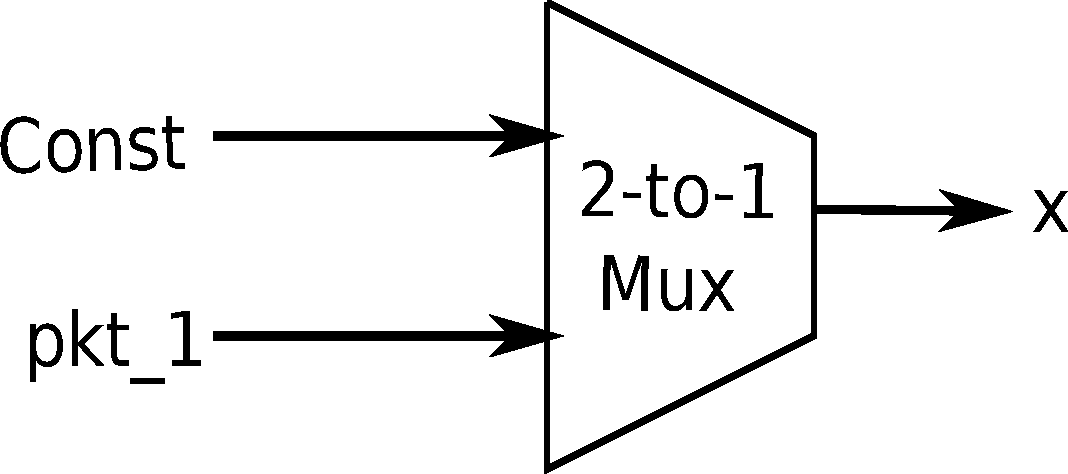
\includegraphics[width=0.2\textwidth]{rw.pdf} & 176 \\
  \hline
  ReadAddWrite (RAW) & 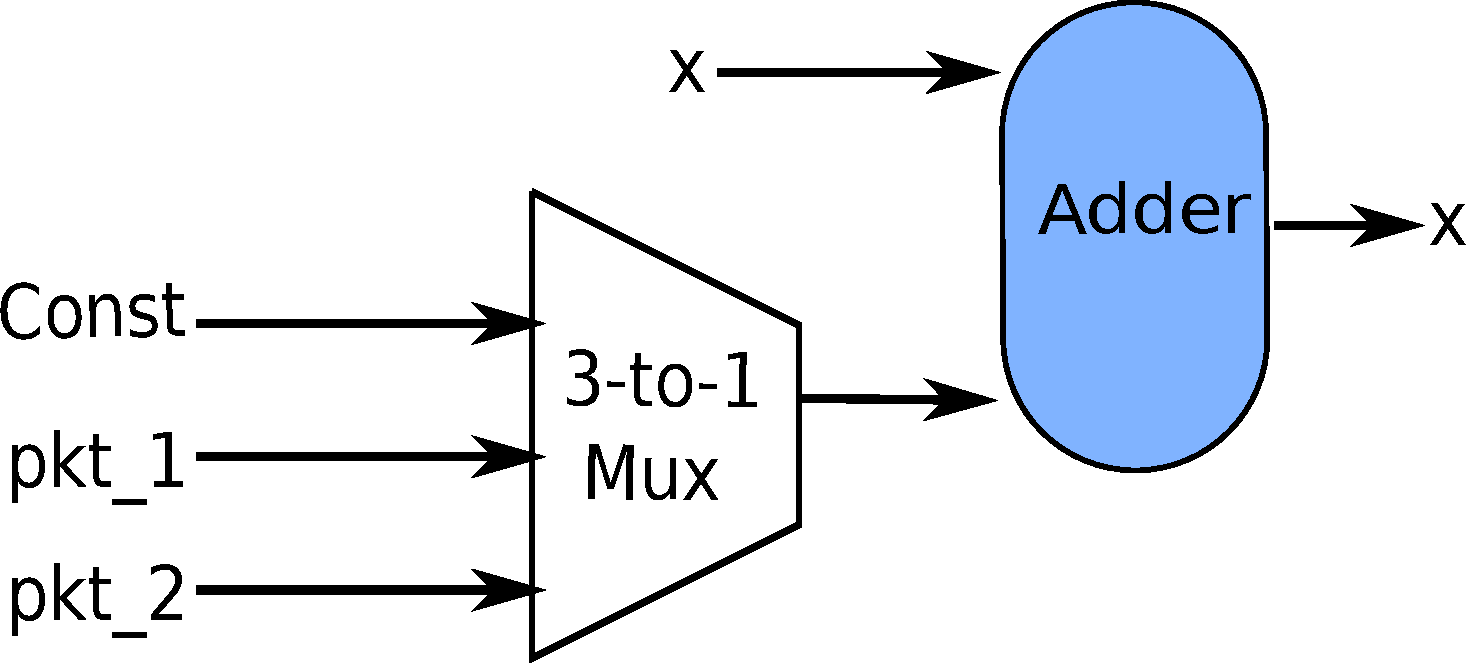
\includegraphics[width=0.2\textwidth]{raw.pdf} & 316\\
  \hline
  \pbox{0.1\textwidth}
  {Predicated\\
  ReadAddWrite (PRAW)} & 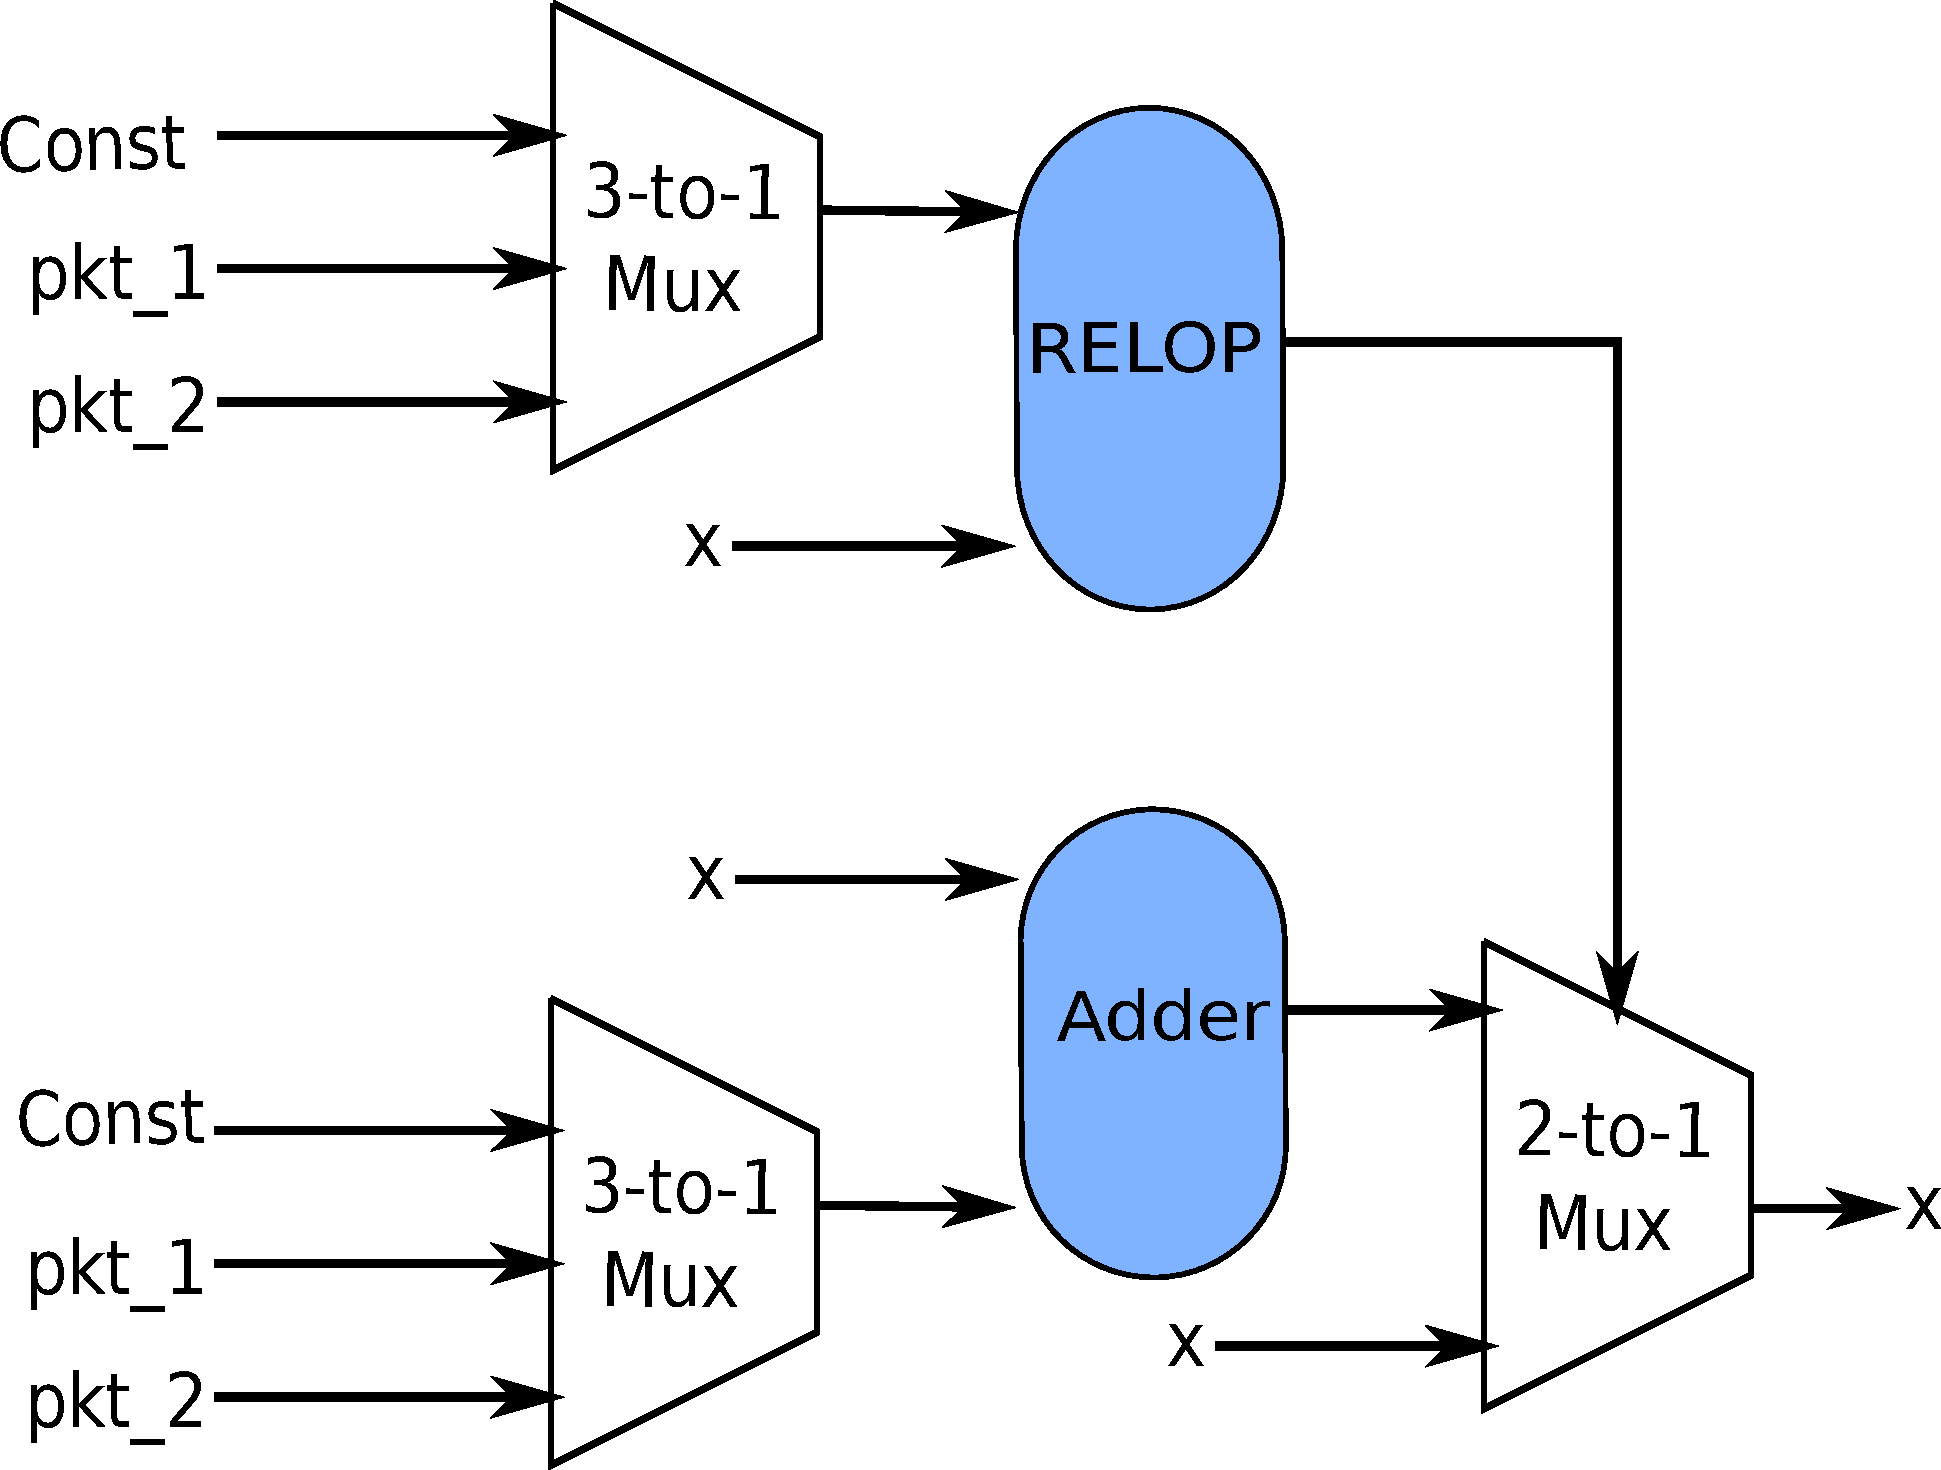
\includegraphics[width=0.3\textwidth]{pred_raw.pdf}  & 393 \\
  \hline
  \end{tabular}
\end{scriptsize}
\caption{Minimum delay of an atom increases with the depth of its circuit. MUX stands
         for a multiplexer, RELOP stands for a relational operation between two operands.}
  \label{tab:circuits}
\end{table}
